\documentclass[a4paper]{article}

\usepackage{placeins}
\usepackage[english]{babel}
\usepackage[utf8x]{inputenc}
\usepackage{amsmath}
\usepackage{amssymb}
\usepackage{float}
\usepackage{graphicx}
\usepackage{wrapfig}
\usepackage[colorinlistoftodos]{todonotes}
\usepackage[authoryear]{natbib}
\usepackage{hyperref}
\usepackage{authblk}
\usepackage[margin=1in]{geometry}
\usepackage{pgfplots}
\pgfplotsset{compat=1.12}
\usepackage{subcaption}


\usepackage[inline,ignoremode]{trackchanges} % Documentation of this package can be found at http:\\trackchanges.sourceforge.net/
\addeditor{MWS} % For each editor, repeat this command with their initials. Monroe is added by default.

\title{Trends and Disparities in Global University Rankings: Insights from Times Higher Education Data}
\author{Rona Guo, Maiqi Hou, Siddhant Sharma, Ziqian Wang, and Yan Xia}
\affil{University of Colorado Boulder}
\affil{STAT 5000: Statistical Methods and Applications I}
\date{December 14, 2023}

\begin{document}

\maketitle

\begin{abstract}
College rankings offer comparative assessments on global higher education institutions' competitiveness and institutional perceptions. This study explores the significance of rankings, disparities in educational quality across nations, and evolving trends in university rankings using the Times Higher Education dataset from 2011 to 2016. The analysis of this data reveals that economic status influences university scores, while class size might impacts teaching quality. Hypothesis tests reveal a significant difference in scores between Chinese and American universities, while the research scores between 2014 and 2015 in the US showed no significant change.
\end{abstract}

\section*{Introduction}
An astonishing number of over 2,000 colleges and universities across the globe are considered in prominent ranking systems, shaping educational aspirations worldwide \cite{marope_rankings_2013}. It is obvious that global university rankings receive attention from students and their parents, but they receive the most attention from governments and universities \cite{sanoff_ussher_massimo_clarke_2007}. Global rankings provide comparative information on the performance of universities in different countries \cite{marope_rankings_2013}, and government follows the global rankings as research universities play a key role in building a country's core competitiveness\cite{hazelkorn_2013}. Likewise, universities are concerned with their rankings, as global rankings are an effective tool for building and maintaining reputation, both of which are important for attracting talent and resources \cite{marope_rankings_2013}.

Looking back at the history of world university rankings, the first university ranking based on surveys and statistics was the publication of ‘America’s Best Colleges’ by the US News \& World Report’ in 1983, which was the first of its kind to compare undergraduate programs in the United States and made this information widely available to the high school population and their parents \cite{marope_rankings_2013}. In addition to the United States, institutions in China and the United Kingdom also publish world university rankings. In 1998, the Chinese leadership declared that the country would have several world-class universities amid a knowledge based economy and was determined to accelerate China’s Moderation. They established the 985 project to build world class universities in China. But what exactly is the definition of a ‘world class university’? This resulted in a ranking of world universities (ARWU) in 2003 \cite{marope_rankings_2013}.  Followed by the release of the Academic Ranking of World Universities(ARWU) by Shanghai Jiao Tong University in 2003 and the Times Higher Education World University Rankings in 2004, the topic has rarely left academia and mainstream media \cite{marope_rankings_2013}.

The criteria and measurement methods of world university rankings are different across different publishers. All mainstream ranking agencies announce the ranking standards with the release of the rankings to ensure the objectivity of the rankings, and even cooperate with well-known research institutions and third party data providers to ensure fairness.  However, major mainstream university ranking organizations have gradually formed their own ranking priorities. Some scholars have discovered that Shanghai Jiao Tong University’s Academic Ranking of World Universities only focuses on research performance\cite{hazelkorn_2013}, while the Times Higher Education rankings strive to fully reflect the activities of global universities, including research, teaching, knowledge transfer and internationalization. The new approach looks at the international mix of faculty and students, research volume, research income and reputation, industry income, and learning environment \cite{marope_rankings_2013}.

Therefore, we used world college ranking data from the Times Higher Education across several years to conduct our analysis. This research aims to delve into three pivotal inquiries. Firstly, it scrutinizes the purpose and significance of college ranking systems, elucidating their crucial role in shaping academic landscapes. Secondly, it investigates the disparities in educational quality across different countries, aiming to unravel the variances and benchmarks in global education. Lastly, it delves into the dynamic nature of ranking distributions over time, seeking to comprehend the evolution and trends within the realm of university rankings.



\section*{Data}

\subsection* {Source}

World university rankings, such as Times Higher Education (THE)\cite{education_2016}, collect data through surveys and publicly available sources, assessing indicators like academic reputation and research output. Data is verified for accuracy, and rankings are based on weighted indicators. Transparency in methodology is key, with rankings published annually or periodically.

\subsection* {Sampling}
The World University ranking dataset under consideration comprises 2603 records spanning the years 2011 to 2016, with 15 fields. 

The dataset employs a set of 13 performance factors as the World University Rankings overall, aggregating the results into five categories as shown in Table 1.

\begin{table}[h]
    \centering
    \caption{Performance measurement effecting the university scores}
    \begin{tabular}{|c|c|}
        \hline
        \textbf{Categories} & \textbf{Factors} \\
        \hline
        Teaching & Learning Environment \\
        \hline
        Research & Volume, Income, Reputation \\
        \hline
        Citation & Research, Influence \\
        \hline
        International Outlook & Staff, Student, and Research \\
        \hline
        Industry Income & Innovation \\
        \hline
    \end{tabular}
\end{table}

Table 2 shows the total number of responses collected by Times Higher Education (THE), per year.

\begin{table}[h]
    \centering
    \caption{Number of Responses}
    \begin{tabular}{|c|c|}
        \hline
        \textbf{Year} & \textbf{Total \# of Responses} \\
        \hline
        2011 & 200 \\
        \hline
        2012 & 402 \\
        \hline
        2013 & 400 \\
        \hline
        2014 & 400 \\
        \hline
        2015 & 401 \\
        \hline
        2016 & 800 \\
        \hline
    \end{tabular}
\end{table}

\subsection* {Key Features}
This paper comprehensively explores key features impacting university rankings, including teaching quality, international reputation, research, citations, industry income, total number of students, student staff ratio, international diversity, and gender ratio.

\subsection* {Bias and Ethics}
It is crucial to recognize any potential biases in the data gathering process while performing this extensive examination of institution rankings using the Times Higher Education dataset. Despite being derived from publicly accessible data and polls, world university rankings could be biassed by factors such as academic reputation that are subjective in nature. Although methodological transparency is essential, biases may arise from things like cultural differences and regional perceptions. Strict monitoring of data cleaning techniques is required due to ethical concerns to remove discrepancies and guarantee the validity and impartiality of the findings reported in this research.

\subsection* {Data Cleaning} 
The data cleaning process involved several essential steps to ensure the accuracy and uniformity of the dataset. Initially, Dataset was loaded using pandas dataframe. 

The female\_male\_ratio column was then divided into male\_ratio and female\_ratio, with each being transformed to a float percentage. Commas were eliminated from the num\_students column, and the \% sign was removed from international\_students to turn it into a float percentage.

To address inconsistencies, the total\_score and income columns were cleansed by replacing - with 0 and converting to float. Additionally, a correction was applied to the country column, rectifying instances of the 'Unted Kingdom' to the 'United Kingdom'. Lastly, any missing values within the dataset were filled with zeros using fillna method, ensuring a comprehensive and consistent dataset for subsequent analysis.

\section*{Methods}
\subsection* {Hypothesis Testing}
We had two hypothesis on this World College Ranking data from 2011 - 2016. First, we conducted paired t test on the mean research score in the United States of America in 2014 and 2015.  Paired t-test is a one sample t-tested in the mean difference and it is a commonly used in social sciences fields to test from before and after effect \cite{hedberg_ayers_2015}. We used a significance level of $\alpha = 0.05$. Since it has only been a year, we believed the mean research score would be very similar.\newline

Hypothesis Test 1:

$$\eta_o: \mu_{USA_{2015}} = \mu_{USA_{2014}}$$
$$\eta_a: \mu_{USA_{2015}} > \mu_{USA_{2014}}$$

Where

$$\mu_{USA_{2014}}: \text{mean of research score in the United States of America in 2014}$$
$$\mu_{USA_{2015}}: \text{mean of research score in the United States of America in 2015} $$\newline


For the second hypothesis, we conducted two sample z test on the average total scores for universities in the United States of America and China in 2015 and set the significance level to $\alpha = 0.05$. We initially assumed there is not a significant difference in the average total score of universities between these two countries as they are both highly developed and leading the world's research in many aspects.\newline 

Hypothesis Test 2:

$$\eta_o: \mu_{China} = \mu_{USA}$$
$$\eta_a: \mu_{China} - \mu_{USA} \neq 0$$

Where\newline 
$$\mu_{USA}: \text{mean of total score for universities in the United States of America in 2015}$$
$$\mu_{China}: \text{mean of total score for universities in China in 2015}$$

\subsection* {Plots Explanation}

\begin{figure}[h]
    \centering
    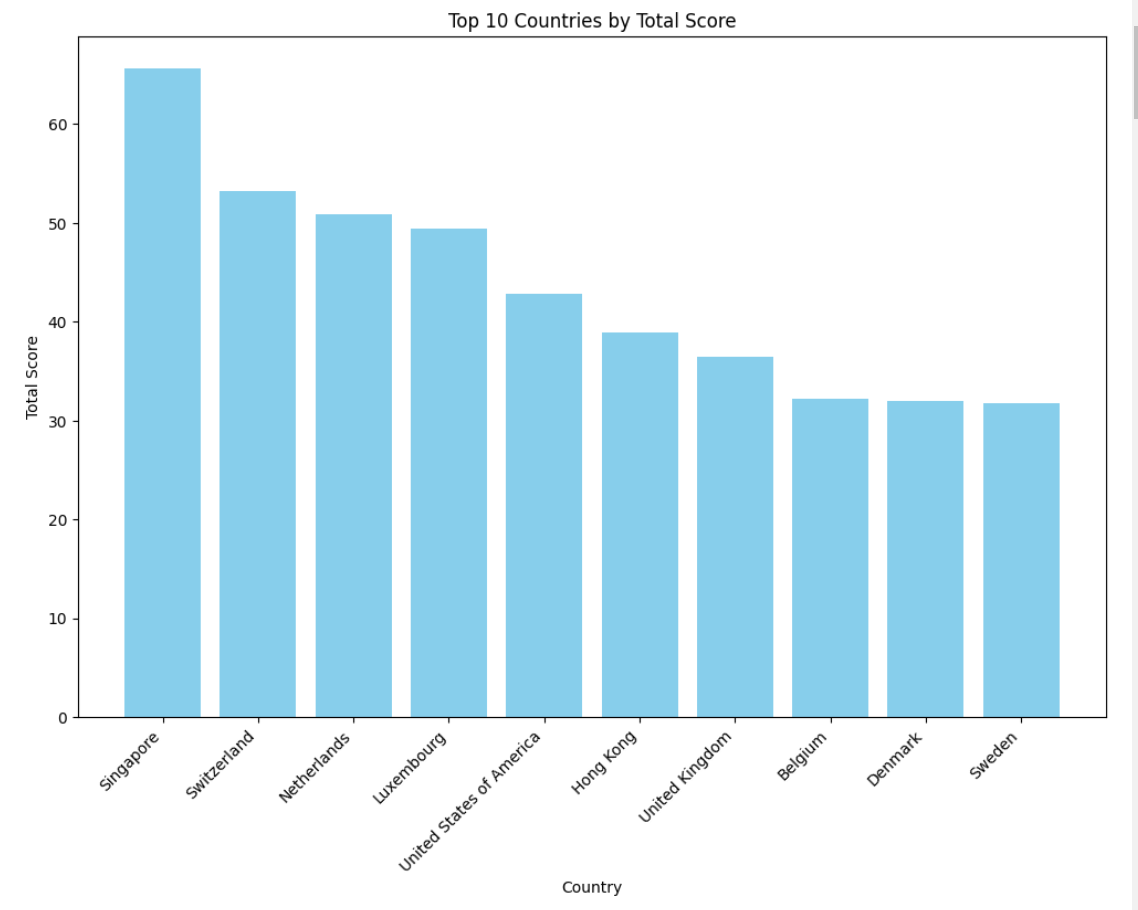
\includegraphics[scale=0.6]{images/WPlot1.png}
    \caption{Top 10 scored countries}
    \label{fig:fig:1}
\end{figure}
\FloatBarrier
Figure~\ref{fig:fig:1} indicates the top 10 countries with the highest average university score. This shows a trend of countries with higher economical level having a higher chance to have better university scores
\begin{figure}[h]
    \centering
    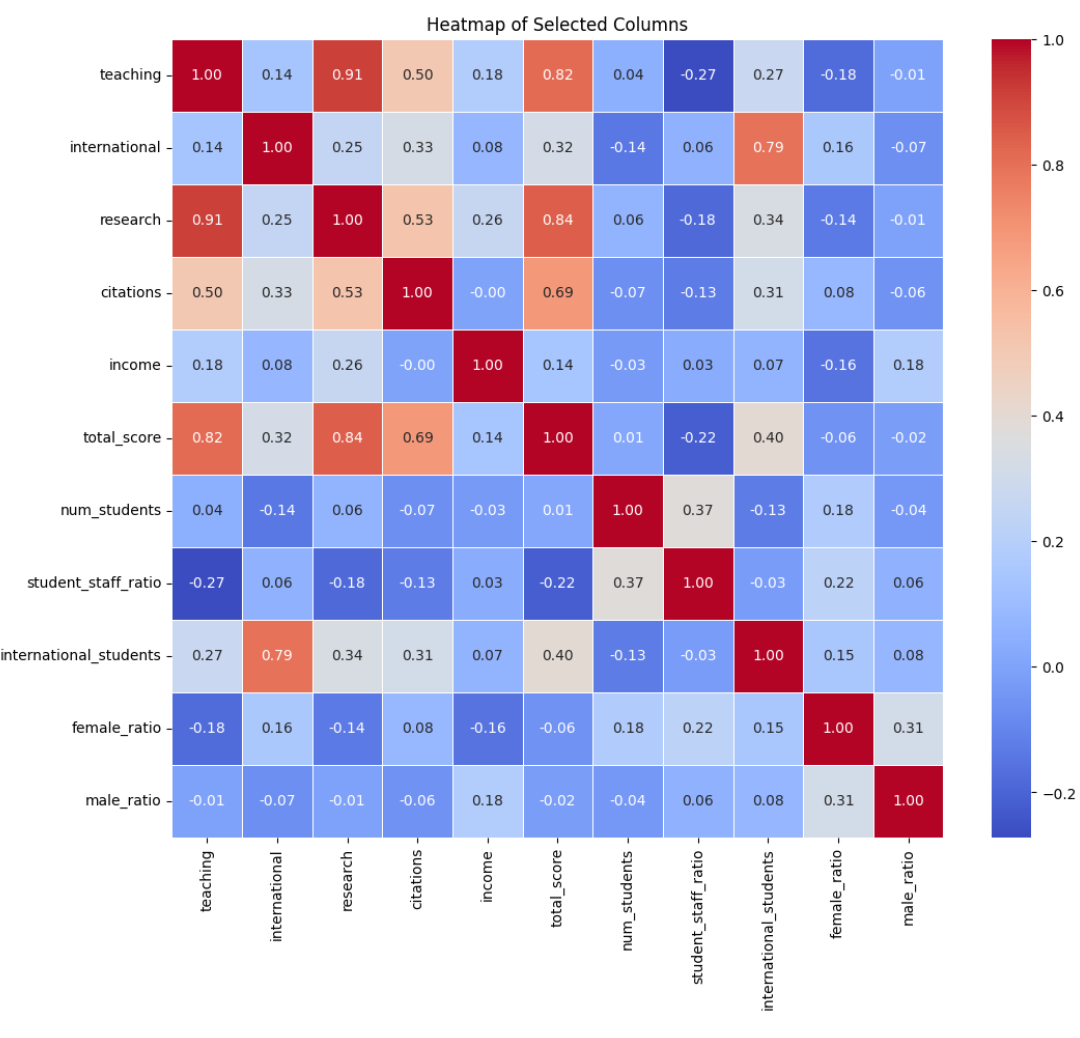
\includegraphics[scale=0.6]{images/WPlot2.png}
    \caption{Correlations between columns}
    \label{fig:fig:2}
\end{figure}
\FloatBarrier
From Figure ~\ref{fig:fig:2} we know that research, teaching and citation have strong correlation between each other. The teaching level has a high effect the total score of a university and male/female ratio is not strongly correlated with other columns, that is, gender ratios does not affect academic standards or the reputation of the school.
\FloatBarrier
\begin{figure}[h]
    \centering
    \begin{subfigure}{\textwidth}
        \centering
        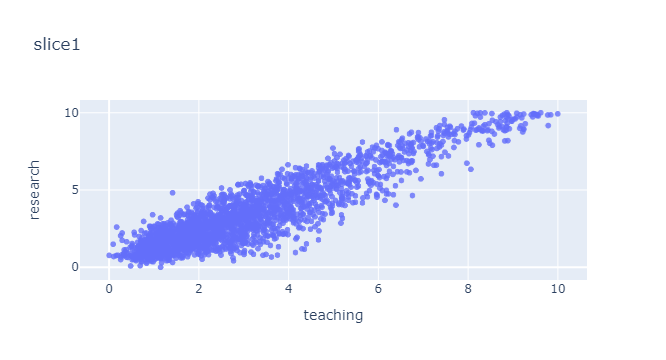
\includegraphics[width=0.7\linewidth]{images/WPlot3.png}
        \caption{3D slice 1}
        \label{subfig:1}
    \end{subfigure}
    \begin{subfigure}{\textwidth}
        \centering
        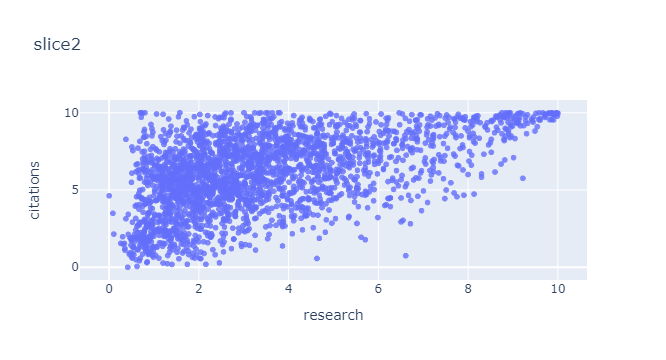
\includegraphics[width=0.7\linewidth]{images/WPlot4.png}
        \caption{3D slice 2}
        \label{subfig:2}
    \end{subfigure}
    \begin{subfigure}{\textwidth}
        \centering
        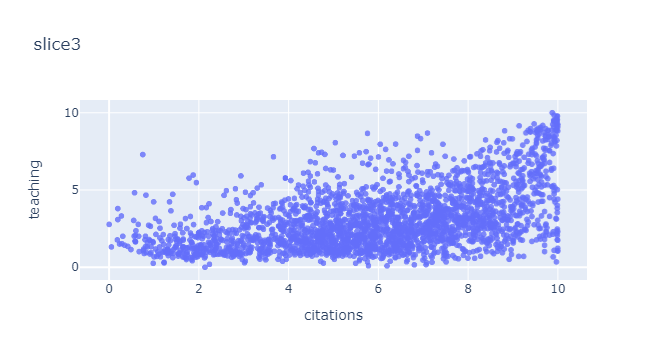
\includegraphics[width=0.7\linewidth]{images/WPlot5.png}
        \caption{3D slice 3}
        \label{subfig:3}
    \end{subfigure}
    \caption{slices of 3d scatter model in 3 different directions}
    \label{fig:fig:3}
\end{figure}

\FloatBarrier
From the correlation heat map we know that teaching, citation and research is strongly correlated but there are more beyond them. From Figure ~\ref{fig:fig:3}, we can see the pairwise relationship between is bound to be cited a lot. There is no university with high teaching standard and low citation level as it seems that students' independent learning can achieve some success in a paper with recognition, but with the support of high-quality teaching, students are more likely to generate more cited papers. On the other hand, when the quality of teaching is low, it is quite difficult to produce a paper that is recognized by others. Research and teaching is highly correlated and there are almost no exceptions.

\FloatBarrier
\begin{figure}[h]
  \centering
  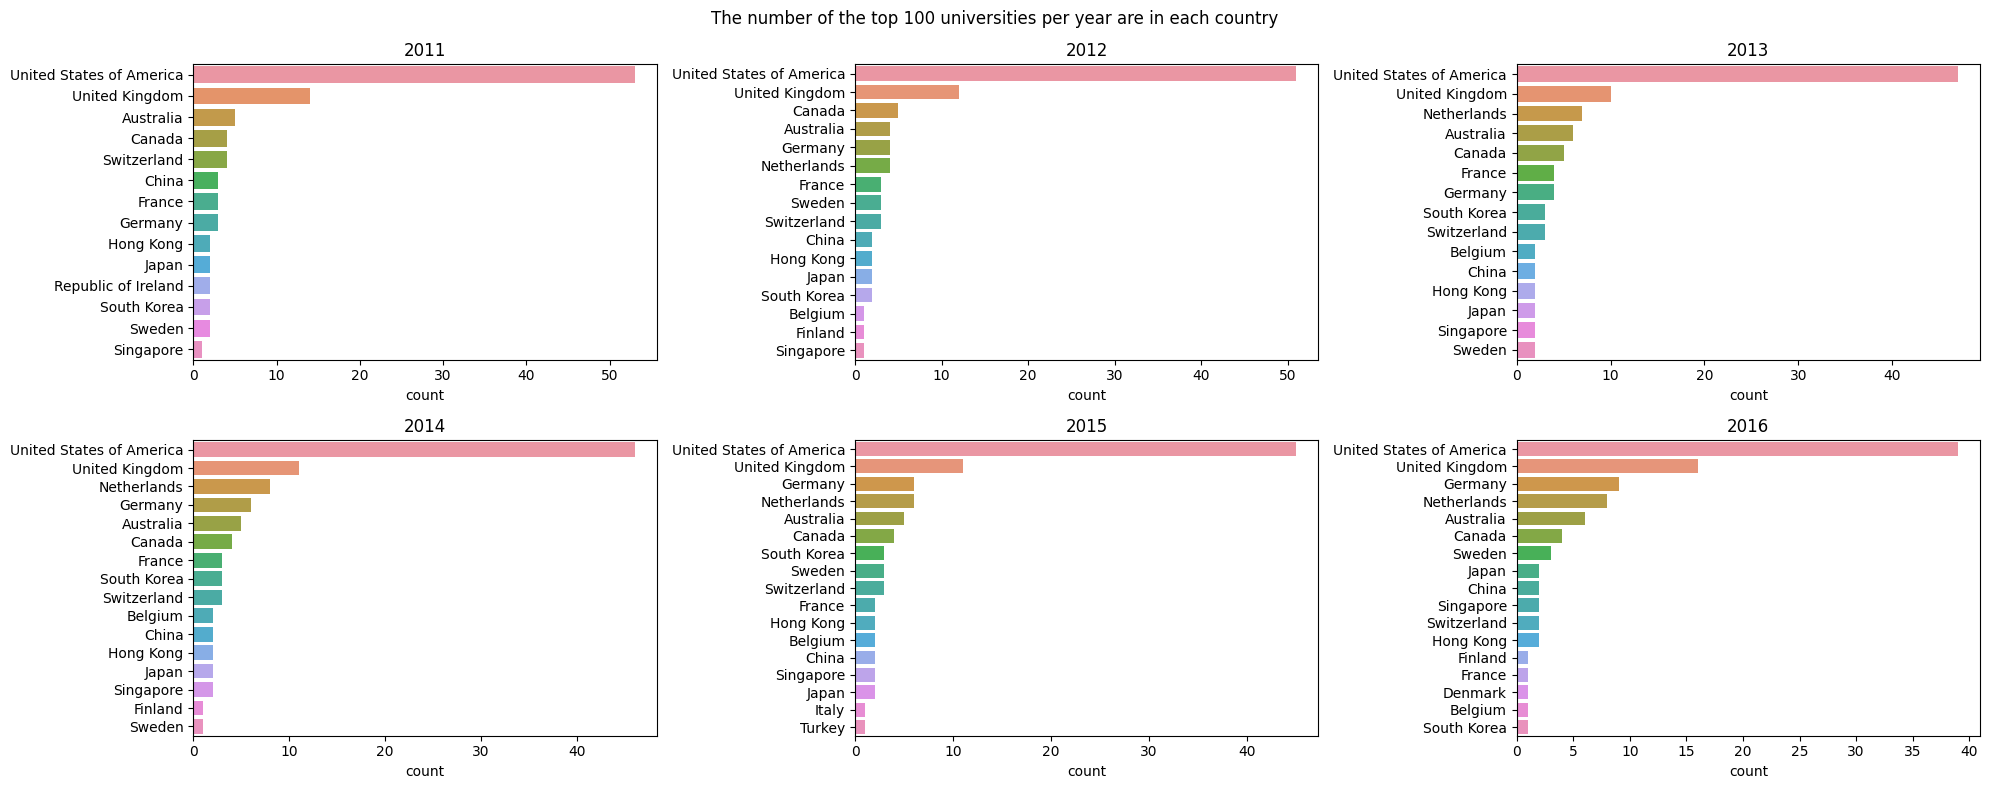
\includegraphics[width=1.0\textwidth]{images/HPlot1.png}
  \caption{The Number of The Top 100 universities per year are in each country}
  \label{fig:4}
\end{figure}
\FloatBarrier
Based on Figure~\ref{fig:4}, it shows clearly the number of top 100 universities in the world in each country during the period from 2011 to 2016. The number of top 100 universities in the United States ranks first position every year, and it outnumbers other countries by three times or four times. The number of top 100 universities in the United Kingdom ranks second. The ranking of the number of universities in the U.S. and the U.K. remained unchanged in the first and second positions during these six years. Australia, Canada, Netherlands, Germany are also ranked high in terms of the number of top 100 universities per year. In addition, the top 100 universities are mostly located in developed countries (except China, which is still a developing country, but it rapidly developed in those years, in the aspect of technology and innovation), and governments of these countries invests more heavily in the funding and equipment in their universities. At the same time, the concepts of science, technology, and innovation in developed countries are also more predominant than other countries, which allows these institutions to work closely with many industries, such as military, finance, space, and high-tech industries. 
\FloatBarrier
\begin{figure}[h]
  \centering
  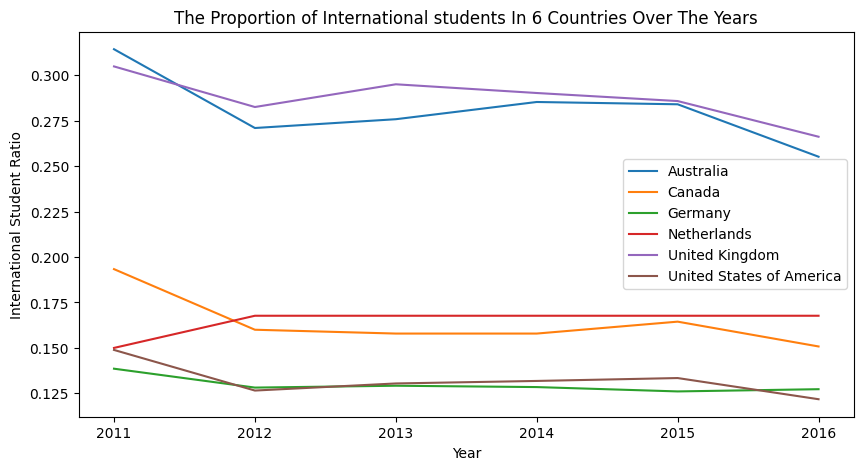
\includegraphics[scale=0.6]{images/HPlot2.png}
  \caption{The Proportion of International Students in 6 Countries Over The Years}
  \label{fig:5}
\end{figure}
\FloatBarrier
According to Figure~\ref{fig:4}, we select the six countries with the highest number of universities in the top 100 in each year. Figure ~\ref{fig:5} shows the average proportion of international students in the United States, the United Kingdom, Germany, Netherlands, Australia, and Canada for each year. We find a high percentage of international students in Australia and the UK compared with the other four countries. Universities in both countries see high amount of applications from international students. One reason is the short-term degree plan in these two countries, with a three-year undergraduate degree or a one-year master's degree. Also, the cost of living and tuition costs may be lower than in other countries. We also find the proportion of international students in each country is decreasing year by year, which may be due to national politics, global economic downturn, or other factors.

\FloatBarrier
\begin{figure}[h]
  \centering
  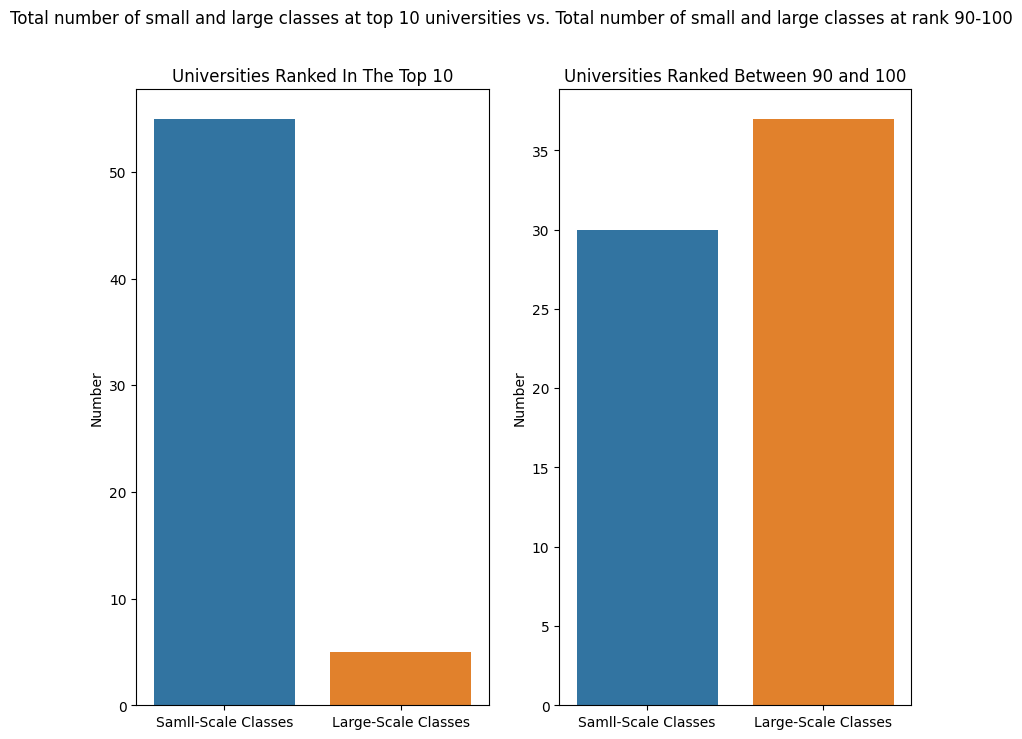
\includegraphics[scale=0.5]{images/HPlot3.png}
  \caption{The Number of Small And Large-scale Classes At Top 10 Universities VS. The Ranked 90-100 Universities}
  \label{fig:6}
\end{figure}
\FloatBarrier
Based on Figure ~\ref{fig:6}, when people are in a class less than 15, we call this the small-scale class. When people are in a class more than 15, it is called the large-scale class. We counted the number of small-scale classes and big-scale classes of Top 10 universities. At the same time, we also counted the number of small classes and large classes of ranked 90-100 universities. We find that the top 10 universities have more the double the number of small-scale classes teaching as the lower ranked universities. The ranked 90-100 universities prefer to use large-scale classes teaching. Therefore, we can infer small-scale classes have better teaching quality, and teaching quality of large-scale class teaching is inferior to that small-scale. 

\section* {Results}
Our first hypothesis test utilized one sample t test (n-1 degree of freedom) for paired testing of mean research scores for universities in the United States between 2014 and 2015. Since the p-value = 0.361 is greater than our $\alpha$ = 0.05, we fail to reject the null hypothesis that the mean research score in the United States in 2015 is equal to the mean research score in the United States in 2014. There is not enough evident to support the alternative hypothesis. \newline Additionally, the second hypothesis test used two sample z test on the mean total score for universities in the  United States and compared it to the mean total score for universities in China in 2015. The p-value = 0.001, which is less than $\alpha$ = 0.05. As a result, we reject the null hypothesis that the mean total score for universities in China and the United States are similar as of 2015 because there is a statistically significant difference in the average score between China and the United States in 2015.

\section*{Discussion}
1. Limitations and future directions: In this study, we only analyzed data from the Times Higher Education's Global University Rankings. Some scholars believe there is little data to support differences between one institution and another, so there are serious concerns about the validity of ranking institutions\cite{davis_2016}. Using only data from the Times Higher Education's Global University Rankings may provide a one-sided judgment on the quality of higher education at different universities. Therefore, we can consider adding other university ranking data to conduct longitudinal comparisons. Lastly, most ranking agencies overly focused on the quality of STEM education, while largely ignoring the liberal arts as it is harder to quantify.

2. Policy implications: In exploring university rankings, we see that university rankings have many impacts on institutional behavior, some of which are not even positive; their role in promoting improvements in academic programs is questionable. In this regard, is it necessary for us to explore whether institutional policies will be adjusted accordingly after university rankings? What is the speed and depth of policy adjustments? Are higher education policies at national or international level affected by university rankings?

3. Educational practice: We can explore the feasibility of specific recommendations based on the findings obtained in this study in subsequent research. That is, explore whether educational institutions can adopt these recommendations to improve their rankings or the quality of their education. For example, based on this study's finding that teaching quality is usually better in smaller classes, it might be recommended that educational institutions move toward smaller class sizes, which would be more feasible for elite private universities than large public universities.

4. Ethical considerations: We should reflect on whether some of the indicators used in rankings may inadvertently encourage practices that may harm educational values or ethics. Discuss the importance of maintaining fairness and integrity during the evaluation process.

\section*{Conclusions}
This research explores the complex dynamics of university rankings to identify the various elements that affect the aggregate ratings of academic institutions. The investigation, which makes use of sophisticated statistical techniques, data visualization hypothesis testing, and rigorous data cleaning, this study aims to provide insights into the complex world of university rankings and the ethical issues that are inherent in these evaluations.

In visualization, university ranking data reveals several key trends: First, wealthier countries tend to have higher-ranked universities, likely due to greater investment in research and innovation. Second, research, teaching, and citation scores are strongly correlated, suggesting a mutually reinforcing cycle of academic excellence. Third, small-scale classes appear to be associated with higher teaching quality compared to large-scale classes. Finally, the proportion of international students is decreasing across most countries, potentially due to political or economic factors. Overall, the findings highlight the complex interplay between economic resources, academic metrics, and teaching methods in shaping university rankings.

In hypothesis testing, we test the difference of the research score within the United States between the adjacent years 2014 and 2015 using paired t-test. Consequently, we failed to reject the null hypothesis, indicating no significant difference in mean research scores between the two years. In contrast, while comparing the average scores of the universities in the United States and China as of 2015 using the 2 sample z-test, we found that there is a significant difference between the two countries' average university scores since the p value was smaller than our alpha level of 0.05.

\clearpage

\bibliographystyle{apalike}
\bibliography{Bibliography}

\end{document}